\documentclass[headinclude,DIV12]{scrartcl}

\usepackage[latin1]{inputenc}
\usepackage[T1]{fontenc}
\usepackage[english]{babel}

\usepackage{scrpage2}
\usepackage{url}
%
\usepackage{pstricks}
\usepackage{pst-optexp}
\let\verPstOptExp\fileversion
\let\datePstOptExp\filedate
\usepackage{multicol}
\usepackage{showexpl}
\lstset{breakatwhitespace}
\usepackage{nicefrac}
\usepackage{graphicx}
\usepackage[colorlinks,linktocpage]{hyperref}
%
% New commands
%
\DeclareRobustCommand\cs[1]{\texttt{\char`\\#1}}
\newcommand{\OptExpPackage}{\textsf{`pst-optexp'}}
\newcommand{\parameter}[1]{\texttt{#1}}
\let\param\textrm
\def\@UrlFont{\small\ttfamily}

%
% Settings
\setkomafont{sectioning}{\normalfont\normalcolor\bfseries}
\setcounter{tocdepth}{2}
%
\makeatletter
\renewenvironment{description}
  {\list{}{\labelwidth\z@ \itemindent-\leftmargin
    \itemsep0pt \parsep0pt
    \let\makelabel\descriptionlabel}}
  {\endlist}
\makeatother
%
% Kopfzeile mit scrpage2 definieren
\clearscrheadfoot
\setheadsepline{0.4pt}
\ihead{\OptExpPackage}\ohead{A PSTricks package to draw optical experimental setups}
\pagestyle{scrheadings}

\psset{subgriddiv=0,griddots=10,gridlabels=7pt}

%%%%%%%%%%%%%%%%%%%%%%%%%%%%%%%%%%%%%%%%%%%%%%%%%%%%%%%%%%%%%%%%%%%%%%%%
\begin{document}
 \title{\texttt{pst-optexp}\\ A PSTricks package to draw optical experimental setups}
 \author{Christoph Bersch \textless
   \href{mailto:usenet@bersch.net}{\texttt{usenet@bersch.net}}\textgreater}
 \date{\datePstOptExp\enspace\enspace Version \verPstOptExp}

\maketitle

\setlength{\columnseprule}{0.6pt}
\begin{multicols}{2}
{\parskip 0pt \tableofcontents}
\end{multicols}
\section{Introduction}
The package \texttt{pst-optexp} is a collection of optical components
that facilitate easy sketching of optical experimental
setups. Mechanisms for proper alignment of different components are
provided internally. This way the user does not have to care for proper
orientation of the elements.

\section{Components}

In the following sections \ref{sec:mirror}--\ref{sec:custom} the
available components with their parameters are described. Up to now
there are two types of components: those which require two reference
points and do not alter the direction of the passing light beam (for
example lenses and retardation plates) and those which work in
reflection and require three reference points (mirrors, grids,
beamsplitters etc.).

In section \ref{sec:general} general parameters are described that are not proprietary
to a specific unit but can be used for several different components. Finally, in
section \ref{sec:labels} the options for the positioning of labels are
explained.

\subsection{Lens}\label{sec:lens}

\begin{description}
\item[\param{lensheight} (dimension):] (\emph{default:~\texttt{1}})
\item[\param{lenswidth} (dimension):] (\emph{default:~\texttt{0.3}})
\item[\param{lenstype} (plainconvex, plainconcave, convexplain, concaveplain, biconvex, biconcave):] (\emph{default:~\texttt{biconvex}})
\item[\param{lensradius} (dimension):] (\emph{default:~\texttt{\cs{empty}}})
\end{description}

For the convex lenses only two parameters are used. If the
parameter \parameter{lensradius} is set, its value will be used together
with \parameter{lensheight} to draw the
lens. Otherwise \parameter{lenswidth} and
\parameter{lensheight} are used. For concave lenses all three parameters
are needed.

\medskip

\begin{LTXexample}[width=3.5cm]
\begin{pspicture}(3,3)\psgrid
  \pnode(0,2){A}
  \pnode(3,1){B}
  \psline[linecolor=green](A)(B)
  \lens[lenstype=plainconvex](A)(B){Lens}
\end{pspicture}
\end{LTXexample}

\bigskip

\begin{LTXexample}[width=3.5cm]
\begin{pspicture}(3,3)\psgrid
  \pnode(0,2){A}
  \pnode(3,1){B}
  \psline[linecolor=green](A)(B)
  \lens[lenstype=convexplain](A)(B){Lens}
\end{pspicture}
\end{LTXexample}

\bigskip

\begin{LTXexample}[width=3.5cm]
\begin{pspicture}(3,3)\psgrid
  \pnode(0,2){A}
  \pnode(3,1){B}
  \psline[linecolor=green](A)(B)
  \lens(A)(B){Lens}
\end{pspicture}
\end{LTXexample}

\bigskip
\begin{LTXexample}[width=3.5cm]
\begin{pspicture}(3,3)\psgrid
  \pnode(0,2){A}
  \pnode(3,1){B}
  \psline[linecolor=green](A)(B)
  \lens[lenstype=plainconcave](A)(B){Lens}
\end{pspicture}
\end{LTXexample}

\bigskip
\begin{LTXexample}[width=3.5cm]
\begin{pspicture}(3,3)\psgrid
  \pnode(0,2){A}
  \pnode(3,1){B}
  \psline[linecolor=green](A)(B)
  \lens[lenstype=concaveplain](A)(B){Lens}
\end{pspicture}
\end{LTXexample}

\bigskip
\begin{LTXexample}[width=3.5cm]
\begin{pspicture}(3,3)\psgrid
  \pnode(0,2){A}
  \pnode(3,1){B}
  \psline[linecolor=green](A)(B)
  \lens[lenstype=biconcave](A)(B){Lens}
\end{pspicture}
\end{LTXexample}

\medskip

\subsection{General plate}

\begin{description}
\item[\param{plateheight} (dimension):] (\emph{default:~\texttt{1}})
\item[\param{platelinewidth} (dimension):] (\emph{default:~\texttt{2\cs{pslinewidth}}})
\end{description}

\medskip

\begin{LTXexample}[width=3.5cm]
\begin{pspicture}(3,3)\psgrid
  \pnode(0,1.5){A}
  \pnode(3,1.5){B}
  \psline[linecolor=green](A)(B)
  \optplate(A)(B){filter}
\end{pspicture}
\end{LTXexample}

\medskip

\subsection{Retardation plate}

\begin{description}
\item[\param{plateheight} (dimension):] (\emph{default:~\texttt{1}})
\item[\param{platewidth} (dimension):] (\emph{default:~\texttt{0.1}})
\end{description}

\medskip

\begin{LTXexample}[width=3.5cm]
\begin{pspicture}(3,3)\psgrid
  \pnode(0,1.5){A}
  \pnode(3,1.5){B}
  \psline[linecolor=green](A)(B)
  \optretplate(A)(B){$\nicefrac{\lambda}{2}$}
\end{pspicture}
\end{LTXexample}

\medskip

\subsection{Pinhole}

\begin{description}
\item[\param{phlinewidth} (dimension):]  (\emph{default~\texttt{2\cs{pslinewidth}}})
\item[\param{owidth} (dimension):] (\emph{default:~\texttt{1}})
\item[\param{iwidth} (dimension):] (\emph{default:~\texttt{0.1}})
\end{description}

\medskip

\begin{LTXexample}[width=3.5cm]
\begin{pspicture}(3,3)\psgrid
  \pnode(0,1.5){A}
  \pnode(3,1.5){B}
  \psline[linecolor=green](A)(B)
  \pinhole(A)(B){PH}
\end{pspicture}
\end{LTXexample}

\medskip

\subsection{Crystal}

\begin{description}
\item[\param{crystalwidth} (dimension):] (\emph{default:~\texttt{2}})
\item[\param{crystalheight} (dimension):] (\emph{default:~\texttt{0.8}})
\item[\param{caxislength} (dimension):] (\emph{default:~\texttt{0.6}})
\item[\param{caxisinv} (boolean):] (\emph{default:~\texttt{false}})
\item[\param{voltage} (boolean):] (\emph{default:~\texttt{false}})
\item[\param{lamp} (boolean):] (\emph{default:~\texttt{false}})
\item[\param{lampscale} (real):] (\emph{default:~\texttt{0.3}})
\end{description}

\medskip

\begin{LTXexample}[width=3.5cm]
\begin{pspicture}(3,3)\psgrid
  \pnode(0,1.5){A}
  \pnode(3,1.5){B}
  \crystal[crystalwidth=1.5,%
           crystalheight=0.6,%
           fillstyle=solid,%
           fillcolor=yellow!90!black,%
           labelangle=-45,%
           voltage,%
           lamp](A)(B){SBN}
  \psline[linecolor=green](A)(B)
\end{pspicture}
\end{LTXexample}

\medskip

\subsection{Box}

\begin{description}
\item[\param{optboxheight} (dimension):] (default:~\texttt{0.5})
\item[\param{optboxwidth} (dimension):] (default:~\texttt{1})
\item[\param{endbox} (boolean):] (default: \texttt{false})
\end{description}

\medskip 

\begin{LTXexample}[width=3.5cm]
\begin{pspicture}(3,3)\psgrid
  \pnode(0,0){A}
  \pnode(3,2){B}
  \psline[linecolor=green](A)(B)
  \optbox[labeloffset=-1](A)(B){Box}
\end{pspicture}
\end{LTXexample}

\bigskip

\begin{LTXexample}[width=3.5cm]
\begin{pspicture}(3,3)\psgrid
  \pnode(0,0){A}
  \pnode(2,2){B}
  \psline[linecolor=green](A)(B)
  \optbox[endbox,labeloffset=1,labelangle=180](A)(B){Box}
\end{pspicture}
\end{LTXexample}

\bigskip

\begin{LTXexample}[width=3.5cm]
\begin{pspicture}(3,3)\psgrid
  \pnode(0,0){A}
  \pnode(2,2){B}
  \psline[linecolor=green](A)(B)
  \optbox[endbox,labelrelative](A)(B){Box}
\end{pspicture}
\end{LTXexample}

\medskip

\subsection{Detector}

\begin{description}
\item[\param{detsize} (dimension):] (default: \texttt{0.5})
\end{description}

\medskip 

\begin{LTXexample}[width=3.5cm]
\begin{pspicture}(3,3)\psgrid
  \pnode(0,0){A}
  \pnode(2,1){B}
  \psline[linecolor=green](A)(B)
  \detector[labeloffset=-1](A)(B){detector}
\end{pspicture}
\end{LTXexample}

\medskip

\subsection{Polarisation}

\begin{description}
\item[\param{pol} (parallel,perp,misc,lcirc,rcirc):] (\emph{default:~\texttt{parallel}})
\item[\param{polwidth} (dimension):] (\emph{default:~\texttt{0.6}})
\end{description}

\medskip

\begin{LTXexample}[width=3.5cm]
\begin{pspicture}(3,3.2)\psgrid
  \pnode(0,0.4){A1}\pnode(3,0.4){B1}
  \pnode(0,1){A2}\pnode(3,1){B2}
  \pnode(0,1.6){A3}\pnode(3,1.6){B3}
  \pnode(0,2.2){A4}\pnode(3,2.2){B4}
  \pnode(0,2.8){A5}\pnode(3,2.8){B5}
  \psline[linecolor=green](A1)(B1)
  \psline[linecolor=green](A2)(B2)
  \psline[linecolor=green](A3)(B3)
  \psline[linecolor=green](A4)(B4)
  \psline[linecolor=green](A5)(B5)
  \polarisation[pol=misc,position=0.2](A5)(B5)
  \polarisation[pol=perp,position=0.35](A4)(B4)
  \polarisation[pol=parallel,position=0.5](A3)(B3)
  \polarisation[pol=rcirc,position=0.65](A2)(B2)
  \polarisation[pol=lcirc,position=0.8](A1)(B1)
\end{pspicture}
\end{LTXexample}

\medskip

%
%
% MIRROR
%
%%%%%%%%%%%%%%%%%%%%%%%%%%%%%%%%%%%%%%%%%%%%%%%%%%%%%%%%%%%%%%%%%%%%%%%%
\subsection{Mirror}\label{sec:mirror}

\begin{description}
\item[\param{mirrorwidth} (dimension):] (\emph{default:~\texttt{1}})
\item[\param{mirrorlinewidth} (dimension):] (\emph{default:~\texttt{0.7\cs{pslinewidth}}})
\item[\param{mirrortype} (normal,piezo,extended):] (\emph{default:~\texttt{normal}})
\item[\param{mirrordepth} (dimension):] (\emph{default:~\texttt{0.08}})
\item[\param{variable} (boolean):] (\emph{default:~\texttt{false}})
\end{description}

The style of the extended mirror is defined as a
psstyle \parameter{ExtendedMirror} and can be changed using
\cs{newpsstyle}. The appearence of the piezo mirror likewise can be
changed by adapting the psstyle \parameter{PiezoMirror}.

\medskip

\begin{LTXexample}[width=3.5cm]
\begin{pspicture}(3,3)\psgrid
  \pnode(0,0){A}
  \pnode(2,2){G}
  \pnode(0,3){B}
  \psline[linecolor=green](A)(G)(B)
  \mirror(A)(G)(B){Mirror}
\end{pspicture}
\end{LTXexample}

\bigskip

\begin{LTXexample}[width=3.5cm]
\begin{pspicture}(3,3)\psgrid
  \pnode(0,0){A}
  \pnode(2,2){G}
  \pnode(0,3){B}
  \psline[linecolor=green](A)(G)(B)
  \mirror[variable](A)(G)(B){Mirror}
\end{pspicture}
\end{LTXexample}

\bigskip

\begin{LTXexample}[width=3.5cm]
\begin{pspicture}(3,3)\psgrid
  \pnode(0,0){A}
  \pnode(2,2){G}
  \pnode(0,3){B}
  \psline[linecolor=green](A)(G)(B)
  \mirror[mirrortype=piezo](A)(G)(B){Piezo}
\end{pspicture}
\end{LTXexample}

\bigskip

\begin{LTXexample}[width=3.5cm]
\begin{pspicture}(3,3)\psgrid
  \pnode(0,0){A}
  \pnode(2,2){G}
  \pnode(0,3){B}
  \psline[linecolor=green](A)(G)(B)
  \mirror[mirrortype=extended,
          mirrordepth=0.1](A)(G)(B){Extended mirror}
\end{pspicture}
\end{LTXexample}

\medskip

\subsection{Beamsplitter}

\begin{description}
\item[\param{bswidth} (dimension):] (\emph{default:~\texttt{1}})
\end{description}

\medskip

\begin{LTXexample}[width=3.5cm]
\begin{pspicture}(3,3)\psgrid
  \pnode(0,2){A}
  \pnode(2,2){G}
  \pnode(3,0){B}
  \psline[linecolor=green](A)(G)(B)
  \beamsplitter(A)(G)(B){BS}
\end{pspicture}
\end{LTXexample}

\medskip


\subsection{Optical grid}

\begin{description}
\item[\param{optgridcount} (integer):] (\emph{default:~\texttt{10}})
\item[\param{optgridwidth} (dimension):] (\emph{default:~\texttt{1}})
\item[\param{optgridheight} (dimension):] (\emph{default:~\texttt{0.1}})
\item[\param{optgriddepth} (dimension):] (\emph{default:~\texttt{0.05}})
\item[\param{optgridlinewidth} (dimension):] (\emph{default:~\texttt{0.7\cs{pslinewidth}}})
\item[\param{reverse} (boolean):] (\emph{default:\texttt{false}})
\end{description}

\medskip

\begin{LTXexample}[width=3.5cm]
\begin{pspicture}(3,3)\psgrid
  \pnode(0,2.5){A}
  \pnode(1.5,2){G}
  \pnode(0,0){B}
  \psline[linecolor=green](A)(G)(B)
  \optgrid(A)(G)(B){grid}
\end{pspicture}
\end{LTXexample}

\bigskip


\begin{LTXexample}[width=3.5cm]
\begin{pspicture}(3,3)\psgrid
  \pnode(0,2.5){A}
  \pnode(1.5,2){G}
  \pnode(0,0){B}
  \psline[linecolor=green](A)(G)(B)
  \optgrid[reverse](A)(G)(B){grid}
\end{pspicture}
\end{LTXexample}

\bigskip

\begin{LTXexample}[width=3.5cm]
\begin{pspicture}(3,3)\psgrid
  \pnode(0,2.5){A}
  \pnode(1.5,2){G}
  \pnode(0,0){B}
  \psline[linecolor=green](A)(G)(B)
  \optgrid[optgridcount=6,%
           optgriddepth=0.2,%
           optgridheight=0.3](A)(G)(B){grid}
\end{pspicture}
\end{LTXexample}

\medskip


\subsection{Custom components}\label{sec:custom}

\begin{LTXexample}[width=3.5cm]
\begin{pspicture}(3,3)\psgrid
  \pnode(0,2){A}
  \pnode(3,1){B}
  \optdipole(A)(B){%
    \rput(0,0){%
      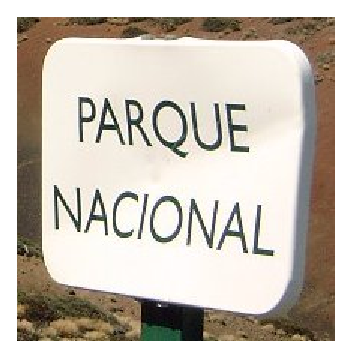
\includegraphics[scale=0.25]{parque-nacional}
    }
  }{Label}
  \psline[linecolor=red](A)(B)
\end{pspicture}
\end{LTXexample}

\bigskip

\begin{LTXexample}[width=3.5cm]
\begin{pspicture}(3,3)\psgrid
  \pnode(0,0){A}
  \pnode(1.5,2){G}
  \pnode(3,1.5){B}
  \opttripole(B)(G)(A){\rput[b](0,0){Text}}{Label}
  \psline[linecolor=red](A)(G)(B)
\end{pspicture}
\end{LTXexample}

\medskip

\subsection{General options}\label{sec:general}

\begin{description}
\item[\param{angle} (real):] (\emph{default:~\texttt{0}})
\item[\param{optional} (boolean):] (\emph{default:~\texttt{false}})
\item[\param{position} (real):] (\emph{default:~\texttt{\cs{empty}}})
\item[\param{abspos} (dimension):] (\emph{default:~\texttt{\cs{empty}}})
\item[\param{showoptdots} (boolean):] (\emph{default:~\texttt{false}})
\end{description}

The parameter \parameter{angle} is available for the macros \cs{optbox}
and \cs{crystal} only, as for the most other cases it would make
no sense. \parameter{optional} can be used with every component and marks it as
optional and can be configured by changing the psstyle \parameter{OptionalStyle}.
\parameter{position} is equivalent to the \parameter{npos} parameter of \cs{ncput},
but is used only for the \lq dipole\rq-macros to position the component
between the two given points. In addition, there is a parameter
\parameter{abspos} that allows absolute positioning between the two line
points. \parameter{showoptdots} shows in black the two points calculated for the
positioning of the component, and in red the reference point for the
label.

\medskip

\begin{LTXexample}[width=3.5cm]
  \begin{pspicture}(3,3)\psgrid
    \pnode(0,1){A}
    \pnode(3,1){B}
    \psline[linecolor=green](A)(B)
    \optbox[labeloffset=-1,%
             angle=10](A)(B){Box}
  \end{pspicture}
\end{LTXexample}

\bigskip

\begin{LTXexample}[width=3.5cm]
  \begin{pspicture}(3,3)\psgrid 
    \pnode(0,1.5){A} 
    \pnode(3,1.5){B}
    \psline[linecolor=green](A)(B) 
    \lens[optional](A)(B){L}
  \end{pspicture}
\end{LTXexample}

\bigskip

\begin{LTXexample}[width=3.5cm]
  \begin{pspicture}(3,3)\psgrid 
    \pnode(0,1.5){A} 
    \pnode(3,1.5){B}
    \psline[linecolor=green](A)(B) 
    \lens[position=0.8](A)(B){L}
  \end{pspicture}
\end{LTXexample}

\bigskip

\begin{LTXexample}[width=3.5cm]
  \begin{pspicture}(3,3)\psgrid 
    \pnode(0,1.5){A} 
    \pnode(3,1.5){B}
    \psline[linecolor=green](A)(B) 
    \lens[abspos=1](A)(B){L}
  \end{pspicture}
\end{LTXexample}

\bigskip

\begin{LTXexample}[width=3.5cm]
  \begin{pspicture}(3,3)\psgrid 
    \pnode(0,0){A} 
    \pnode(1.5,2){G}
    \pnode(0,3){B} 
    \psline[linecolor=green](A)(G)(B)
    \mirror[labelangle=0,showoptdots](A)(G)(B){Mirror}
  \end{pspicture}
\end{LTXexample}

\medskip

\subsection{Labels}\label{sec:labels}

\begin{description}
\item[\param{labeloffset} (dimension):] (\emph{default:~\texttt{1}})
\item[\param{labelangle} (real):] (\emph{default:~\texttt{-90}})
\item[\param{labelstyle} (macro):] (\emph{default:~\texttt{\cs{small}}})
\item[\param{labelalign} (\cs{rput} pos string):] (\emph{default:~\texttt{c}})
\item[\param{labelrelative} (boolean):] (\emph{default:~\texttt{false}})
\end{description}

\parameter{labeloffset} specifies the offset from the center of the component, \parameter{labelangle} is the
absolute angle which is independent of the component orientation, 
\parameter{labelstyle} is the textstyle that is used to typeset the
label and \parameter{labelalign} corresponds to the refpoint of
\cs{rput}. With \parameter{labelrelative} the label is oriented like the
component is.

\newpage
\section{Examples}
\begin{LTXexample}[pos=t,vsep=10mm]
\begin{pspicture}(12,2.4)\psgrid
\pnode(1,1.2){CCD}\pnode(12,1.2){Start}
\psline[linewidth=2\pslinewidth,linecolor=green!90!black](Start)(CCD)
\psset{plateheight=1.5,
       lensheight=1.5,
       lensradius=2}
\polarisation[pol=perp,
              position=0.1](Start)(CCD)
\optretplate[position=0.15](Start)(CCD){$\nicefrac{\lambda}{2}$}
\lens[lensheight=0.5,
      lensradius=0.5,
      position=0.25](Start)(CCD){$L_1$}
\lens[position=0.5](Start)(CCD){$L_2$}
\optplate[position=0.57,
       labelangle=90,
       platelinewidth=3\pslinewidth](Start)(CCD){SLM}
\optplate[position=0.63,
       labelangle=270](Start)(CCD){PF}
\lens[position=0.7](Start)(CCD){$L_3$}
\optbox[endbox](Start)(CCD){CCD}
\end{pspicture}
\end{LTXexample}

\begin{LTXexample}[pos=t,vsep=10mm]
\begin{pspicture}(6,3.5)
  \psgrid[subgriddiv=1,griddots=10,gridlabels=7pt]
  \psset{labelstyle=\scriptsize}
  \pnode(1.5,1){LaserOut}
  \pnode(3,1){Grid}
  \pnode(6,3){Out}
  \pnode(4,3){Mvar}
  \psline[linewidth=2\pslinewidth,
         linecolor=red!90!black](LaserOut)(Grid)(Out)\psline(Grid)(Mvar)
  \optbox[endbox,optboxwidth=1.5](Grid)(LaserOut){diodelaser}
  \optretplate[position=0.3,
               labeloffset=0.7](LaserOut)(Grid){$\nicefrac{\lambda}{4}$}
  \optgrid[labeloffset=0.5](LaserOut)(Grid)(Out){grid}
  \mirror[variable,
          labelangle=20,
          labeloffset=1](Grid)(Mvar)(Grid){variable mirror}
\end{pspicture}
\end{LTXexample}

\psset{unit=1cm}
\begin{LTXexample}[pos=t,vsep=10mm]
\begin{pspicture}(9,6)\psgrid
  \pnode(1.5,5){Laser}\pnode(4,5){PBS}\pnode(6.5,5){PBS2}
  \pnode(6.5,5.7){piezo}\pnode(4,2){BSFwd}\pnode(6.5,2){BSBwd}
  \pnode(2,2){BS4f}\pnode(2,0.5){M4f3}\pnode(8,2){M4f1}
  \pnode(8,0.5){M4f2}\pnode(1,2){CCD}
  \psline[linecolor=green!90!black,linewidth=2\pslinewidth]%
         (Laser)(PBS2)(piezo)(BSBwd)(M4f1)(M4f2)(M4f3)(BS4f)(CCD)
  \psline[linecolor=green!90!black,linewidth=2\pslinewidth](PBS)(BSFwd)(BS4f)
  \psset{mirrorwidth=0.6, plateheight=0.7, owidth=0.7, labeloffset=0.6, labelstyle=\scriptsize, lensheight=0.8, lenswidth=0.2, bswidth=0.5} 
  \optbox[endbox,optboxwidth=1.5, optboxheight=0.7]%
     (PBS)(Laser){\parbox{1.5cm}{\centering Nd:YAG\\ 532\,nm}}
  \lens[lensheight=0.5, position=0.2](Laser)(PBS){MO}
  \pinhole[position=0.3, labelangle=90](Laser)(PBS){PH}
  \lens[position=0.5](Laser)(PBS){L}
  \optretplate[position=0.8](Laser)(PBS){$\nicefrac{\lambda}{2}$}
  \beamsplitter[labelangle=90](Laser)(PBS)(BSFwd){PBS}
  \optretplate[labelangle=180](PBS)(BSFwd){$\nicefrac{\lambda}{2}$}
  \lens[position=0.8,labelangle=180](PBS)(BSFwd){L}
  \optretplate(PBS)(PBS2){$\nicefrac{\lambda}{2}$}
  \beamsplitter[labelangle=0](PBS)(PBS2)(piezo){PBS}
  \optretplate[labelangle=180, abspos=0.5](PBS2)(piezo){$\nicefrac{\lambda}{4}$}
  \mirror[mirrortype=piezo, labelangle=0](PBS2)(piezo)(PBS2){PZ}
  \lens[position=0.8,labelangle=0](PBS2)(BSBwd){L}
  \beamsplitter(PBS)(BSFwd)(BSBwd){BS}
  \beamsplitter(PBS2)(BSBwd)(BSFwd){BS}
  \crystal[crystalwidth=1, crystalheight=0.5, voltage, lamp, fillstyle=solid, fillcolor=yellow!90!black, labeloffset=0.8](BSFwd)(BSBwd){SBN:Ce}
  \mirror[labelangle=0](BSBwd)(M4f1)(M4f2){M}
  \mirror[labelangle=0](M4f1)(M4f2)(M4f3){M}
  \lens(M4f2)(M4f3){L}
  \mirror[labelangle=180](M4f2)(M4f3)(BS4f){M}
  \beamsplitter[labelangle=90](M4f3)(BS4f)(CCD){BS}
  \optbox[endbox](BS4f)(CCD){CCD}
  \lens[abspos=0.7](BSFwd)(BS4f){L}
  \lens[abspos=0.7](BSBwd)(M4f1){L}
  \psline[linecolor=green!90!black, linewidth=2\pslinewidth](BSFwd)(BSBwd)
\end{pspicture}
\end{LTXexample}

\section{Known bugs}
 
For some reason, filling of the concave lenses by
specifiying \parameter{fillstyle} does not work properly. For sure there
are other bugs, but they are not known, yet. If you find some, do not
hesitate to contact me.

\section{ Todo}

\begin{itemize}
\item Add components for fiber optics.
\end{itemize}

Drawing of extended beams with focusing, and so on, is not planned to be
integrated in the near future due to missing ideas for the realization.


\end{document}
